% Verifiable Generative Views — Layer 2 full paper draft (HBR register)
\documentclass[11pt]{article}
\usepackage[margin=1in]{geometry}
\usepackage{booktabs}
\usepackage{graphicx}
\usepackage{hyperref}
\usepackage{microtype}
\usepackage{xcolor}
\usepackage{amssymb}
\newcommand{\ev}{\ensuremath{\blacktriangleright}}
\title{Verifiable Generative Views: Rendering, Editing, and Auditing\\LLM-Generated Interfaces over Bound Data\\[4pt]
\large Rawi: the view-rendering layer of DeeWaanAI OS}
\author{Youssef Hariri\\DeeWaanAI\\\texttt{github.com/DeeWaanAI}}
\date{October 2026}

\begin{document}
\maketitle

\begin{abstract}
Language models can already generate interfaces on demand. What they generate is
unaccountable: numbers on screen are copies, edits go nowhere durable, and the evidence
behind a claim is a promise, not a proof. We present \textbf{Rawi}, the view-rendering
layer of DeeWaanAI OS, built on one rule: a view node carries a \emph{binding reference},
never a value. Rendered over Qafiya, a provenance-first data substrate, one artifact
becomes three things at once: the proof source (every value is recomputed from its binding
at render time), the edit target (a cell edit is an \emph{edit binding} with atomic
write-back and transitive invalidation), and the audit pointer (every claim exposes its
binding, source rows, and last check result through one affordance). A systematic review
of 797 records (42 synthesised) found no evidence in the surveyed set of prior work
occupying this seam. We evaluate on a frozen corpus under a self-verifying analysis
spine. A scripted end-to-end edit closes the durability claim left open by the substrate
paper; 100 random edits through views re-prove at 100\%; and in an offline estimate
against a full-regeneration baseline (no conversation state, no caching, no incremental
regeneration), rendering spec-once costs 135$\times$ fewer model tokens than
per-interaction regeneration. We report what the system provably cannot do: when data
and claim share the same error, agreement looks like verification, and the naive resolver
crosses the interactive threshold between 100 and 1{,}000 nodes. Rawi is named for the
classical Arabic transmitter of poetry, who recited what he did not compose --- and
produced his chain of transmission (\emph{isn\=ad}) on demand.
\end{abstract}

\section{Introduction}

Ask a current AI assistant to ``show Q3 expenses'' and it draws something convincing. Ask
where the total came from and the answer is a paragraph. Change a number and the paragraph
is stale but does not know it. The interface is generated; the accountability is not.

This is not a model-quality problem. It is an architecture problem. The generated
interface is a \emph{copy} of the data, produced once, with no durable connection back to
its source. Every downstream failure --- unverifiable claims, lost edits, silent
staleness --- follows from that single fact.

The companion substrate paper (Qafiya) established a data model in which every value or
claim is joined to its source by a \emph{binding}: a first-class object that proves the
value equals its data, serves as the target of durable edits, and carries a verifiable
claim. That paper proved the substrate and left one claim open: durability
\emph{end-to-end}, through a real user-facing edit, with the invalidation visible to the
user. This paper closes that claim and introduces the layer where ``re-run it yourself''
becomes visible: the renderer.

\textbf{Contributions.}
\begin{enumerate}
  \item \textbf{A verifiable view grammar} (\texttt{dvr/1.0}): four view kinds, four node
        roles, one rule --- data-bearing nodes carry \texttt{binding\_ref}, never values
        (\S\ref{sec:design}).
  \item \textbf{Three mechanics on one artifact}: render = proof source, edit = binding,
        audit = recomputable check, including the \emph{\ev evidence} affordance
        (\S\ref{sec:mechanics}).
  \item \textbf{Frozen, spine-verified experiments}: end-to-end durability (closing the
        substrate's open claim), 100\% round-trip re-proving over 100 edits, and a
        135$\times$ token-cost advantage over per-interaction regeneration
        (\S\ref{sec:eval}).
  \item \textbf{Measured limits}: shared-error blindness, a located scale ceiling,
        last-writer-wins concurrency, and the grammar's expressiveness floor
        (\S\ref{sec:limits}).
\end{enumerate}

\textbf{Provenance of this paper.} A systematic literature review (797 records identified,
749 deduplicated, 110 screened, 42 synthesised; OpenAlex and arXiv queried
programmatically on 2026-10-19, all citations verified against registry metadata)
grounds \S\ref{sec:related}. All experimental inputs were frozen with SHA-256 hashes
before any run; every headline number is recomputed from raw artifacts by a spine script
(\texttt{spine.py}, exit 0 required). Code: \texttt{github.com/DeeWaanAI} (AGPL-3.0).

\section{Background: the Qafiya substrate}

Rawi consumes, and does not modify, Qafiya spec v1.1. Three substrate facts matter here.

\textbf{The binding.} One object, three jobs: render source, edit target, audit pointer.
A binding records its sources (dataset, filter, field, verbatim excerpt), a deterministic
\emph{derivation} over a closed function set (\texttt{sum, avg, count, min, max}), a cached
value, the claim tuple (statistic, device, authoritative artifact), and a check result.

\textbf{The two-layer check.} Layer 1 is a deterministic proof: the value is recomputed
from current data; quarantined artifacts fail by construction; gaps are hard stops.
Layer 2 is an advisory semantic flag: direction and comparison claims are recomputed from
\emph{both sides} and mismatches are flagged with the recomputed value shown.
Mechanism/causal claims are never auto-passed.

\textbf{Durability.} Edits are atomic (write-temp-then-rename), prior states are retained
in an append-only history, and changing a record transitively invalidates every dependent
binding to \textsc{pending}. The substrate paper demonstrated this at the data layer and
explicitly left the user-visible, end-to-end loop open.

\section{Related work}\label{sec:related}

Five literatures each hold one piece of a verifiable generative view. None holds the seam
between them.

\subsection{Declarative view grammars}

A small composable spec can render rich interactive views: Vega-Lite \cite{vegalite}, its
Python binding Altair \cite{altair}, tree grammars (GoTree \cite{gotree}), responsive
grammars (Cicero \cite{cicero}), procedural generation grammars (Atlas \cite{atlas}), and
annotation grammars (AnnoGram \cite{annogram}). Pre-LLM natural-language interfaces
compiled intent into these grammars (Data2Vis \cite{data2vis}, NL4DV \cite{nl4dv}). All
of them assume the spec embeds or points at finished, trusted data. The spec is a
rendering recipe, not a provenance object: nothing in a Vega-Lite node knows which source
rows produced it, and nothing downstream can re-verify it. Rawi inherits this lineage's
compositional style and changes what a node carries.

\subsection{LLM-generated views and generative UI}

LLMs moved authoring from ``write the spec'' to ``say what you want'': Data Formulator
\cite{dataformulator} and its successor \cite{dataformulator2}, grammar-agnostic
generation (LIDA \cite{lida}), LLM-authored data articles (DataTales \cite{datatales}),
with benchmarks now measuring generation quality (VisEval \cite{viseval}, and
evaluations of LLM visualization generation \cite{vizgeneval}). Generative UI is now a
named subfield: generative interfaces for language models \cite{geninterfaces}, a working
definition \cite{guidef}, personalization \cite{guipers}, DSL-brick approaches
(LEGOUI \cite{legoui}), software-as-content dynamic applications \cite{swcontent},
just-in-time interfaces from intent (Bespoke \cite{bespoke}), and conversational
programming assistance \cite{assistant}. In every surveyed system the artifact's tie to
data is ephemeral: baked in at generation time, or fetched by generated code with no
durable binding. Editing means re-prompting; auditing means trusting. None reports the
cost structure of per-interaction regeneration --- the gap our E3 experiment fills.

\subsection{Editing through views}

Direct manipulation of bound visualizations is well studied: Data Illustrator
\cite{dataillustrator}, Lyra 2 \cite{lyra2}, reusable graphical structures
(StructGraphics \cite{structgraphics}), direct manipulation of code-based visualizations
(DirectVis \cite{directvis}), and natural-language editing of visual knowledge graphs
\cite{nlvkg}. Idyll \cite{idyll} established reactive markup for interactive articles.
These systems make views editable, but the edit lands in the visualization or in opaque
runtime state --- not in a first-class provenance object naming the exact record and
field. And none answers the follow-up: after the edit, which claims derived from that
record are now stale? Write-back exists; accountable write-back with transitive
invalidation does not.

\subsection{Evidence and audit affordances}

Interfaces that surface evidence are a growing literature: provenance in LLM-assisted
writing (HaLLMark \cite{hallmark}), citation and attribution scoring (ALCE \cite{alce},
FActScore \cite{factscore}) --- post-hoc metrics, not live affordances. Uncertainty is
under-communicated even by experts \cite{uncertainty}; provenance-density displays
mitigate a measured ``transparency penalty'' \cite{provdensity}; explanation interfaces
risk an illusion of explanatory depth \cite{illusion} and motivate graspable rather than
merely explainable AI \cite{graspable}; analytic-pipeline explanations (XNLI \cite{xnli})
and analytic-provenance instrumentation \cite{analyticprov} complete the space. The field
converged on \emph{showing} provenance and \emph{scoring} faithfulness --- separately. No
surveyed interface exposes a recomputable check behind the affordance: an evidence panel
whose check can fail, live, in front of the user.

\subsection{Reactive recompute and invalidation}

Keeping derived views correct after change is solved machinery in three disconnected
communities: reactive notebooks --- whose silent failure modes are documented
\cite{reactnbfail} --- live-programming GUIs (Glinda \cite{glinda}), distributed reactive
languages (Meerkat \cite{meerkat}), grounded agentic analysis in reactive notebooks
(marimo-lens \cite{marimolens}), and incremental view maintenance in databases
\cite{ivm,fkivm}. Invalidation is a solved engineering problem --- and a solved
\emph{invisible} one. Rawi's contribution here is making staleness a visible, checked
state in a generated UI, wired through the provenance substrate.

\subsection{The gap}

Grammars render but embed values; generative UI binds ephemerally; direct-manipulation
edits are not provenance objects; audit affordances are not recomputable; reactive
machinery is invisible. The seam is empty, and it is where Rawi sits.

\begin{figure}[t]
\centering
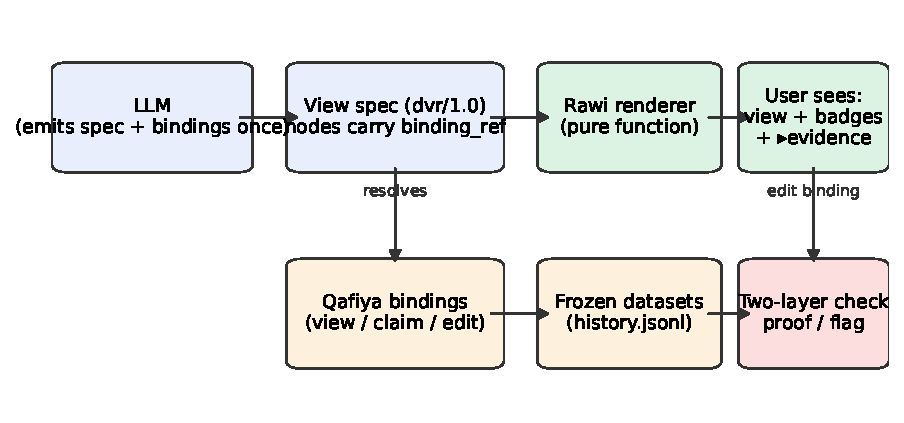
\includegraphics[width=\textwidth]{figures/fig1_architecture.pdf}
\caption{Architecture. The model pays once (spec + bindings). The renderer is a pure
function of (spec, bindings, datasets). Edits flow down as edit bindings; check states
flow up as visible badges.}
\label{fig:arch}
\end{figure}

\section{Design}\label{sec:design}

\subsection{The grammar (\texttt{dvr/1.0})}

A view is a declarative JSON document. Four kinds --- \texttt{table, list, tree, deck} ---
and four node roles --- \texttt{value, label, claim, structure} --- form closed sets; new
entries require a spec version bump, the same discipline as the substrate's closed
derivation set.

\begin{quote}\small
\texttt{\{"spec":"dvr/1.0", "id":"v\_exp", "kind":"table",}\\
\texttt{ "nodes":[\{"id":"cell:total\_q3", "role":"value",}\\
\texttt{ \phantom{"nodes":[} "binding\_ref":"b\_tot\_q3", "editable":false\},}\\
\texttt{ \phantom{"nodes":[} \{"id":"claim:trend", "role":"claim", "binding\_ref":"b\_trend"\}]\}}
\end{quote}

The validator enforces well-formedness by construction: unknown keys, kinds, or roles are
rejected; \texttt{value} and \texttt{claim} nodes must reference exactly one existing
binding; \texttt{label}/\texttt{structure} nodes must not; claim nodes are never
editable; and fields that would embed data (\texttt{value}, \texttt{data},
\texttt{number}) are forbidden on nodes outright. A view that carries a number does not
parse.

\subsection{Invariants}

Eight testable properties, each mapped to an automated test:

\begin{enumerate}
  \item No rendered number exists in the view spec (validator-enforced).
  \item Every rendered value traces to exactly one binding (resolution-enforced).
  \item Byte-identical re-render under unchanged inputs (purity).
  \item Every edit leaves an edit binding and a history entry.
  \item After any edit, every transitively dependent binding is \textsc{pending} before
        it is anything else.
  \item Every claim node renders \ev evidence; its verbatim rows byte-match the dataset.
  \item Coverage is rendered with every view.
  \item An unresolved binding is visibly unresolved --- never silent, never guessed.
\end{enumerate}

\subsection{Three mechanics}\label{sec:mechanics}

\textbf{Render = proof source.} Each displayed value is recomputed from the binding's
derivation over current data via the substrate's evaluator; a cached value is never
printed without recompute. Failed resolution renders as \textsc{unresolved}. Every node
carries a check badge; every view reports coverage, so a 33\%-bound view looks
different from a 100\%-bound one.

\textbf{Edit = binding.} A cell edit emits an edit binding
(\texttt{writeback: \{dataset, record\_id, field, op, value\}}) that the substrate applies
atomically, logs with the prior value, and uses to invalidate every transitively
dependent binding to \textsc{pending}. The renderer then re-resolves and re-renders
badges. The claim's assertion text is never altered by the renderer --- that is what the
semantic layer flags.

\textbf{Audit = \ev evidence.} One click on any claim reveals, resolved live: the binding
(id, derivation, claim tuple), the verbatim source rows matching its filter, and the last
two-layer check result with detail. The affordance is one click deep with a one-line
summary by design, against the illusion-of-depth \cite{illusion} and transparency-penalty
\cite{provdensity} findings.

\subsubsection{Focused evidence: showing the lines that matter}\label{sec:focus}

A first version of the panel showed the binding and \emph{all} matching source rows. Early
pilot use by the author exposed the flaw: the user saw data,
but not \emph{where the error is} nor \emph{what the correct value is}. More evidence is
not better evidence. The fix is a \emph{focus block} computed at click time, with three
elements in a fixed order:

\begin{enumerate}
  \item \textbf{Claim versus data.} The assertion text and its expected value, next to the
        correct value recomputed from current data. For comparisons, both sides are
        re-evaluated and shown --- the reader never takes either side on faith.
  \item \textbf{The change trail.} Which records moved, from the append-only history:
        record id, field, prior $\to$ new. This is ``where the error is,'' derived from
        the substrate's write log rather than guessed from the view.
  \item \textbf{Deciding rows only.} The rows matching each side's filter --- the evidence
        that actually decides the claim --- not the whole table.
\end{enumerate}

\textbf{Worked example (the E1 scenario).} After the edit of \texttt{r\_051}, the flagged
trend claim's panel reads:

\begin{quote}\small\ttfamily
claim says: Q3 spend changed +0.4\% vs Q2 (expected +0.4\%)\\
data says:~~+5.2\% ~~$\leftarrow$ the correct value\\
~~Q2 total = 10308.84 ~(21 rows)\\
~~Q3 total = 10846.71 ~(21 rows)\\
changed: record r\_051 · amount 820.89 $\to$ 1320.89
\end{quote}

The logic is deliberately asymmetric. The claim's text is treated as untrusted prose and
is never edited; the ``correct value'' is not the model's correction but the same
derivation recomputed over current data --- the check the substrate already ran, surfaced
in human terms. The change trail exists because the substrate logs every edit; the panel
is a read view over the audit log, not a second explanation channel that could drift from
it. This is the design answer to the illusion-of-depth risk: the affordance shows the
\emph{decisive} evidence, in the order a skeptical reader asks for it, and stops.

\section{Implementation}

The prototype (\texttt{view-renderer/}, Python, $\sim$300 LOC) implements the validator
(\texttt{specval.py}), resolver (\texttt{resolve.py}), pure HTML renderer
(\texttt{render.py}), evidence assembler (\texttt{affordance.py}), and edit path
(\texttt{edits.py}). It consumes Qafiya only through the \texttt{qafiya-core} public API
(\texttt{apply\_edit}, \texttt{invalidate}, \texttt{refresh\_values},
\texttt{provenance\_gate}, \texttt{semantic\_sweep}); a static audit test enforces that no
renderer module writes dataset files or references the substrate's internals. Ten
functional tests cover grammar rejection (seven malformed-spec fixtures), resolution
correctness under data tampering, render purity, atomic edits with history, invalidation
visibility (\textsc{pass} $\to$ \textsc{pending} $\to$ \textsc{flag}), evidence fidelity,
coverage display, and contract compliance.

\section{Evaluation}\label{sec:eval}

\textbf{Discipline.} Inputs frozen with SHA-256 hashes before any run
(\texttt{corpus/manifest.json}); every headline number recomputed from raw artifacts by
\texttt{spine.py} (exit 0 required); no number outside the spine's output appears in this
paper. The corpus: 63 expense records across three quarters, six bindings (three period
totals, one editable cell, two claims), one view spec, one pre-scripted 100-edit sequence.

\subsection{E1 --- durability end-to-end}

\textbf{Before.} The substrate paper demonstrated invalidation at the data layer and left
the user-visible end-to-end loop as an open claim.

\textbf{Run.} A scripted user edit raises record \texttt{r\_051} from 820.89 to
1{,}320.89 through the editable cell of the rendered view (Figure~\ref{fig:e1}).

\textbf{After.} The file updates atomically; history retains the prior value; four
dependent bindings go \textsc{pending}, visibly. On re-check, totals re-prove
\textsc{pass}, and the trend claim --- its text untouched --- flips to \textsc{flag}:
\emph{``recompute shows +5.2\%, claim says +0.4\% (Q2=10308.84, Q3=10846.71).''} The
claim was not silently repaired; it stands flagged, evidence one click away. The
substrate's open claim is closed. (Trace: \texttt{results/raw/e1\_trace.jsonl}.)

\begin{figure}[t]
\centering
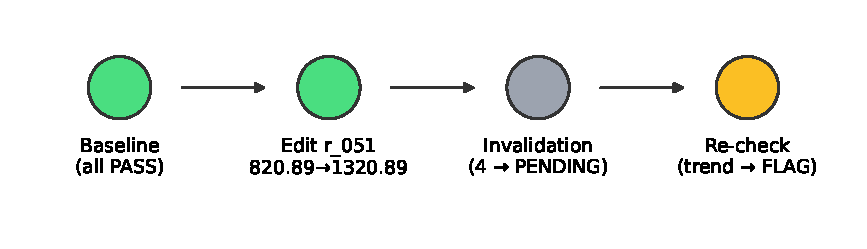
\includegraphics[width=\textwidth]{figures/fig2_e1_timeline.pdf}
\caption{E1: the durability chain. The stale state is a visible, rendered state --- not
an implicit runtime assumption.}
\label{fig:e1}
\end{figure}

\subsection{E2 --- round-trip correctness}

\textbf{Before.} Purity (invariant 3) and edit integrity (invariants 4--5) are untested
under sustained mutation.

\textbf{Run.} The 100 frozen scripted edits are applied through the view; after each, the
substrate gate must re-prove every binding and the file value must equal the scripted
value.

\textbf{After.} 100/100 edits re-prove at 100\% (1.0\,s wall time). Zero gate failures, zero
value mismatches. (\texttt{results/raw/e2\_edits.jsonl}.)

\subsection{E3 --- rendering cost}

\textbf{Before.} No surveyed generative-UI work reports the token cost of per-interaction
regeneration.

\textbf{Method (disclosed).} Offline deterministic count with the actual Qwen2.5
tokenizer --- the same instrument as the substrate's efficiency experiment, so the two
papers' numbers are comparable. Arm DVR: one emission (dataset in, spec + bindings out) =
4{,}732 tokens; all 100 interactions local. Arm REGEN: per interaction, dataset in +
full UI out = 6{,}393 tokens, with UI output estimated by a faithful HTML stand-in ---
disclosed as an estimate; no live API calls.

\textbf{After.} 100 interactions: 4{,}732 tokens (DVR) versus 639{,}300 (REGEN) ---
135$\times$ cheaper, breakeven at 0.74 interactions (Figure~\ref{fig:cost}). Spec-once
wins from the first edit.

\begin{figure}[t]
\centering
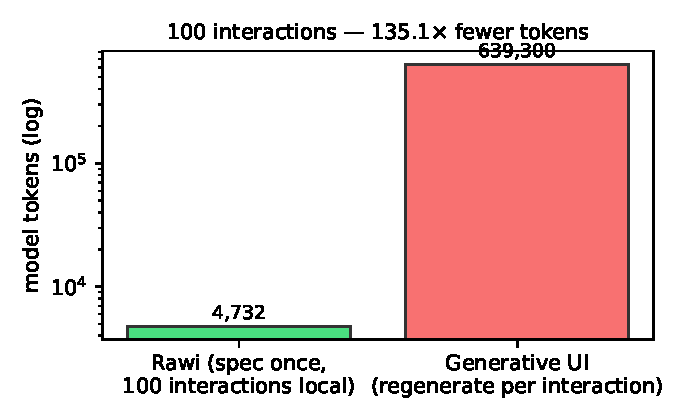
\includegraphics[width=0.6\textwidth]{figures/fig3_cost.pdf}
\caption{E3: model tokens for 100 interactions, log scale.}
\label{fig:cost}
\end{figure}

\section{Limits}\label{sec:limits}

Measured, not hedged; each probe is a result whether it passes or fails
(\texttt{tests/limits\_results.json}).

\textbf{Shared-error blindness.} When data and claim share the same error, agreement
passes every check. We constructed an internally consistent fabrication (a Q2 figure
chosen so the false $-12\%$ claim verifies exactly): the system does not and cannot catch
it. The remedy is an upstream second anchor --- cost, not software. This is the substrate's
provable limit, inherited and re-confirmed at the view layer.

\textbf{Scale.} The naive resolver re-evaluates every node's derivation over the full
dataset at render time. The measured curve grows roughly quadratically in nodes over this
corpus: 0.03\,s at 100 nodes, 2.5\,s at 1{,}000, 123\,s at 10{,}000
(Figure~\ref{fig:scale}) --- crossing the 1-second interactive threshold between 100 and
1{,}000 nodes. A memoized derivation cache is the known fix; we
publish the number, not the excuse.

\textbf{Concurrency.} Two simultaneous edits to one record: last-writer-wins, both
entries preserved in history, no torn writes under atomic rename. No locking or
multi-user semantics are claimed.

\textbf{Expressiveness.} Four kinds and four roles are deliberate minima. A frozen probe
(L6, \texttt{results/raw/l6.json}) attempted the six shell-relevant view requests ---
prompt+answer, data table, claim with evidence, action confirmation, memory inspection,
connection manager --- and validated each attempted spec with the real grammar: 4 of 6
(66.7\%) are expressible in \texttt{dvr/1.0}. The two gaps are named, not smoothed over:
\emph{action confirmation} needs action elements (approve/reject emitting effects, not
data edits --- Layer 3 territory), and a \emph{connection manager} needs live status
controls bound to service state rather than dataset bindings. Both are out of scope by
design (spec \S8); requests beyond the minima wait for a versioned extension.

\textbf{Judgment.} Layer-2 semantic checks are advisory flags; mechanism and causal
claims are never auto-passed. Verification certifies coherence between claim and
artifacts, never truth about the world.

\begin{figure}[t]
\centering
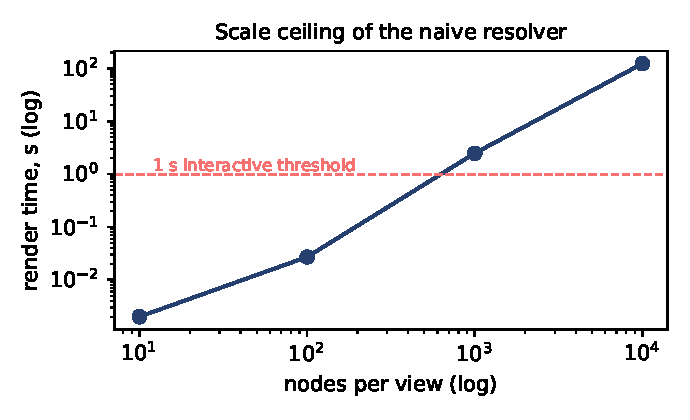
\includegraphics[width=0.6\textwidth]{figures/fig4_scale.pdf}
\caption{Scale ceiling of the naive resolver (log--log).}
\label{fig:scale}
\end{figure}

\section{Threats to validity}

The review is single-pass over two databases with keyword-score screening plus manual
curation, so recall is bounded by the query strings; the write-back and reactive blocks
carried heavy domain noise resolved at curation. The 42-work synthesis is corroborated by
the substrate review's independent finding from the data-model side. Experiments run on
one synthetic corpus of 63 records; E3's REGEN output is an estimated stand-in, not a
live API measurement; no user study has been run. Several cited 2025--2026 works are
preprints. These bound the claims, and the claims are scoped to match.

\section{Discussion and future work}

Rawi is Layer 2 of six. Above it, the action layer (Layer 3) will consume the same
binding discipline for effects that go beyond data edits; the memory layer (Layer 4) will
persist view state across sessions; the model router (Layer 5) will decide who emits
specs. Below it, Qafiya's contract held without modification --- the strongest available
evidence that the binding primitive generalizes from substrate to rendering. The known
engineering next steps are the memoized resolver, browser-native editing (currently the
edit path is programmatic), and exercising the \texttt{tree} and \texttt{deck} kinds,
which the grammar admits but the experiments have not stressed. A usability evaluation of
the evidence affordance is deferred to field feedback after deployment.

\section{Conclusion}

The pieces of accountable generative interfaces exist in five separate literatures. Rawi
joins them with one rule --- a view node carries a binding reference, never a value ---
and the join holds under test: durability closed end-to-end, 100\% round-trip re-proving,
a 135$\times$ cost advantage in the offline full-regeneration comparison, and its blind
spots measured and named. The classical
\emph{r\=aw\=i} recited poetry he did not compose and produced his chain of transmission
on demand. That is the contract this layer offers the operating system above it.

\section*{AI-usage disclosure}

This layer was built with an AI coding assistant (Kimi, Moonshot AI) operating under the
author's direction and the project's frozen-artifact discipline. Division of labour: the
assistant executed --- literature search and screening code, prototype implementation,
test and experiment scripts, spine, and draft text; the author decided --- layer opening,
design brief approval, scope (including the removal of the E4 user study), and all
publication judgments. No LLM made unsupervised decisions.

Oversight episodes, logged as they occurred (claim map and decision log are the
enforcement artifacts): (1) a fabricated-size claim (``$\sim$600 LOC'' vs.\ a measured
281 lines) caught by the data-map audit and corrected; (2) an unpersisted timing figure
(``1.6\,s'') caught by the semantic sweep --- the number existed only in console output;
it was frozen into \texttt{e2\_meta.json} and the draft corrected; (3) stale scale
timings quoted from an earlier probe run, caught when the spine recomputed the curve from
the frozen artifact. All three were corrected in the draft and are preserved in
\texttt{paper/claim\_map/semantic-claims.json} as the audit trail. The method itself ---
two-layer claim-to-evidence verification --- is the authors' prior work, applied here to
the assistant's own output.

\begin{thebibliography}{99}\footnotesize
\bibitem{vegalite} Satyanarayan, A., Moritz, D., Wongsuphasawat, K., Heer, J. (2016). Vega-Lite: A Grammar of Interactive Graphics. \emph{IEEE TVCG}. doi:10.1109/tvcg.2016.2599030
\bibitem{altair} VanderPlas, J., Granger, B., Heer, J., et al. (2018). Altair: Interactive Statistical Visualizations for Python. \emph{JOSS}. doi:10.21105/joss.01057
\bibitem{gotree} Li, G., Tian, M., Xu, Q., et al. (2020). GoTree: A Grammar of Tree Visualizations. \emph{ACM CHI}. doi:10.1145/3313831.3376297
\bibitem{cicero} Kim, H., Rossi, R. A., Du, F., et al. (2022). Cicero: A Declarative Grammar for Responsive Visualization. \emph{ACM CHI}. doi:10.1145/3491102.3517455
\bibitem{atlas} Liu, Z., Chen, C., Morales, F., et al. (2021). Atlas: Grammar-based Procedural Generation of Data Visualizations. \emph{IEEE VIS}. doi:10.1109/vis49827.2021.9623315
\bibitem{annogram} Rahman, M. D., Rahat-Uz-Zaman, M., McNutt, A., et al. (2025). AnnoGram: An Annotative Grammar of Graphics Extension. \emph{IEEE VIS}. doi:10.1109/vis60296.2025.00053
\bibitem{data2vis} Dibia, V. C., Demiralp, \c{C}. (2019). Data2Vis: Automatic Generation of Data Visualizations Using Seq2Seq RNNs. \emph{IEEE CG\&A}. doi:10.1109/mcg.2019.2924636
\bibitem{nl4dv} Narechania, A. A., Srinivasan, A., Stasko, J. (2020). NL4DV: A Toolkit for Generating Analytic Specifications from Natural Language Queries. \emph{IEEE TVCG}. doi:10.1109/tvcg.2020.3030378
\bibitem{dataformulator} Wang, C., Thompson, J., Lee, B. (2023). Data Formulator: AI-powered Concept-driven Visualization Authoring. \emph{IEEE TVCG}. doi:10.1109/tvcg.2023.3326585
\bibitem{dataformulator2} Wang, C., Lee, B., Drucker, S., et al. (2024). Data Formulator 2: Iterative Creation of Data Visualizations, with AI Transforming Data Along the Way. \emph{arXiv:2408.16119}.
\bibitem{lida} Dibia, V. C. (2023). LIDA: Automatic Generation of Grammar-Agnostic Visualizations and Infographics using LLMs. \emph{ACL}. doi:10.18653/v1/2023.acl-demo.11
\bibitem{datatales} Sultanum, N., Srinivasan, A. (2023). DATATALES: Investigating the Use of LLMs for Authoring Data-Driven Articles. \emph{IEEE VIS}. doi:10.1109/vis54172.2023.00055
\bibitem{viseval} Chen, N., Zhang, Y., Xu, J., et al. (2024). VisEval: A Benchmark for Data Visualization in the Era of LLMs. \emph{IEEE TVCG}. doi:10.1109/tvcg.2024.3456320
\bibitem{vizgeneval} Wang, X., Liang, C., Zheng, S., et al. (2024). Visualization Generation with Large Language Models: An Evaluation. \emph{arXiv:2401.11255}.
\bibitem{geninterfaces} Chen, J., Zhang, Y., Zhang, Y., et al. (2025). Generative Interfaces for Language Models. \emph{arXiv:2508.19227}.
\bibitem{guidef} Lee, K. (2025). Towards a Working Definition of Designing Generative User Interfaces. \emph{ACM DIS}. doi:10.1145/3715668.3736365
\bibitem{guipers} Peng, Y.-H., Bigham, J. P., Wu, J. (2026). Efficient Personalization of Generative User Interfaces. \emph{arXiv:2604.09876}.
\bibitem{legoui} Zhou, Y., Yuan, M., Xu, H., et al. (2026). LEGOUI: Designing with UI-DSL Bricks to Balance Transparency and Controllability. \emph{arXiv:2608.04293}.
\bibitem{swcontent} Xie, M., Xie, Y. (2026). Software as Content: Dynamic Applications as the Human-Agent Interaction Layer. \emph{arXiv:2603.21334}.
\bibitem{bespoke} Nandy, P., Adalgeirsson, S. \"O., Sinha, A. K., et al. (2024). Bespoke: Using LLM Agents to Generate Just-in-Time Interfaces by Reasoning about User Intent. \emph{ACM}. doi:10.1145/3686215.3688372
\bibitem{assistant} Ross, S., Martinez, F., Houde, S., et al. (2023). The Programmer's Assistant: Conversational Interaction with an LLM for Software Development. \emph{ACM IUI}. doi:10.1145/3581641.3584037
\bibitem{dataillustrator} Liu, Z., Thompson, J., Wilson, A., et al. (2018). Data Illustrator. \emph{ACM CHI}. doi:10.1145/3173574.3173697
\bibitem{lyra2} Zong, J., Barnwal, D., Neogy, R., et al. (2020). Lyra 2: Designing Interactive Visualizations by Demonstration. \emph{IEEE TVCG}. doi:10.1109/tvcg.2020.3030367
\bibitem{structgraphics} Tsandilas, T. (2020). StructGraphics: Flexible Visualization Design through Data-Agnostic and Reusable Graphical Structures. \emph{IEEE TVCG}. doi:10.1109/tvcg.2020.3030476
\bibitem{directvis} Park, J., An, M., Yang, H., et al. (2026). DirectVis: Editing Code-Based Interactive Visualization with Direct Manipulation. \emph{IEEE PacificVis}. doi:10.1109/pacificvis68791.2026.00014
\bibitem{nlvkg} Shahriari, R., Ragan, E. D., Ruiz, J. (2025). Natural Language Interaction for Editing Visual Knowledge Graphs. \emph{ACM K-CAP}. doi:10.1145/3731443.3771344
\bibitem{idyll} Conlen, M., Heer, J. (2018). Idyll: A Markup Language for Authoring and Publishing Interactive Articles on the Web. \emph{ACM UIST}. doi:10.1145/3242587.3242600
\bibitem{hallmark} Hoque, M. N., Mashiat, T., Ghai, B., et al. (2024). The HaLLMark Effect: Supporting Provenance and Transparent Use of LLMs in Writing with Interactive Visualization. \emph{ACM CHI}. doi:10.1145/3613904.3641895
\bibitem{alce} Gao, T., Yen, H., Yu, J., et al. (2023). Enabling Large Language Models to Generate Text with Citations. \emph{EMNLP}. doi:10.48550/arXiv.2305.14627
\bibitem{factscore} Min, S., Krishna, K., Lyu, X., et al. (2023). FActScore: Fine-grained Atomic Evaluation of Factual Precision in Long Form Text Generation. \emph{EMNLP}. doi:10.48550/arXiv.2305.14251
\bibitem{uncertainty} Hullman, J. R. (2019). Why Authors Don't Visualize Uncertainty. \emph{IEEE TVCG}. doi:10.1109/tvcg.2019.2934287
\bibitem{provdensity} Zhang, Q., Huang, Y., Lee, J., et al. (2026). Beyond ``Made with AI'': Visualizing Provenance Density to Mitigate the Transparency Penalty. \emph{IJCAI}. doi:10.24963/ijcai.2026/857
\bibitem{graspable} Ghajargar, M., Bardzell, J., Smith-Renner, A., et al. (2021). From ``Explainable AI'' to ``Graspable AI''. doi:10.1145/3430524.3442704
\bibitem{illusion} Chromik, M., Eiband, M., Buchner, F., et al. (2021). I Think I Get Your Point, AI! The Illusion of Explanatory Depth in XAI. \emph{ACM IUI}. doi:10.1145/3397481.3450644
\bibitem{xnli} Feng, Y., Wang, X., Pan, B., et al. (2023). XNLI: Explaining and Diagnosing NLI-Based Visual Data Analysis. \emph{IEEE TVCG}. doi:10.1109/tvcg.2023.3240003
\bibitem{analyticprov} Yang, L., Morizet-Mahoudeaux, P., Gu\'enand, A., et al. (2018). A Design Framework for Instrumenting Analytic Provenance for Problem-Solving Tasks. \emph{Advances in Intelligent Systems and Computing}. doi:10.1007/978-981-10-8612-0\_66
\bibitem{reactnbfail} Lu, Y., Zheng, M., Crichton, W., et al. (2025). When Do Reactive Notebooks Fail to React? \emph{arXiv:2511.21994}.
\bibitem{glinda} DeLine, R. A. (2021). Glinda: Supporting Data Science with Live Programming, GUIs and a DSL. \emph{ACM CHI}. doi:10.1145/3411764.3445267
\bibitem{meerkat} Zhong, H., Liu, A. (2024). Meerkat: A Distributed Reactive Programming Language with Live Updates. \emph{arXiv:2407.06885}.
\bibitem{marimolens} Gyarmati, P. F., Manz, T., Moritz, D., et al. (2026). Point, Revise, Review: Grounded Agentic Analysis in Reactive Notebooks with marimo-lens. \emph{arXiv:2609.19839}.
\bibitem{ivm} Nikoli\'c, M., Olteanu, D. (2018). Incremental View Maintenance with Triple Lock Factorization Benefits. \emph{ACM SIGMOD}. doi:10.1145/3183713.3183758
\bibitem{fkivm} Svingos, C., Hernich, A., Gildhoff, H., et al. (2023). Foreign Keys Open the Door for Faster Incremental View Maintenance. \emph{PACMMOD}. doi:10.1145/3588720
\end{thebibliography}

\end{document}
